Ahora procederemos a analizar, experimentar y discutir los métodos que conciernen al rankeo de páginas Web. Recordemos que en este trabajo se utilizó el modelo PageRank para modelar el rankeo de páginas web utilizando cadenas de Markov y se implementó una versión optimizada especialmente para este problema, presentada en \cite{Kamvar2003}

\subsubsection{Convergencia de PageRank}
Para los experimentos de velocidad de convergencia y rendimiento en general de PageRank utilizamos los datasets de \cite{SNAP}. Para eso, elegimos tres datasets de diferentes tamaños y coeficiente de conectividad \footnote{Con esto nos referimos a que tan conectado está el grafo, esto puede medirse por ejemplo como $\frac{2e}{v(v-1)}$, donde $e$ son las aristas del grafo y $v$ los vertices, dado que el grafo completo tiene $\frac{v(v-1)}{2}$ aristas.}, web-Stanford, web-NotreDame y web-Google.

\begin{figure}[H]
\centering
\begin{tabular}{| c | c | c |}
  \hline
  Dataset & Vértices & Aristas \\ \hline \hline
  web-Stanford & 281.903 & 2.312.497 \\ \hline
  web-NotreDame & 325.729 & 1.497.134 \\ \hline
  web-Google & 916.428 & 5.105.039 \\ \hline
\end{tabular}
\end{figure}


Lo primero que se puede decir de este Datasets es que la diferencia de cantidad de vértices de cada uno nos va a permitir analizar como varía según el tamaño de la red. 

Además, notemos como el dataset web-Stanford está mucho más conectado que el dataset web-NotreDame, dado que tiene menos vértices pero más aristas. Creemos que esto va a impactar negativamente en la performance, dado que sobre una red poco conectada el algoritmo va a converger más rápido.

Eso se puede notar fácilmente si se piensa en el grafo que es totalmente disconexo. En ese caso, todas las entradas de la matriz van a valer $\frac1n$, y el método de la potencia va a converger en un paso.

Otra cosa que podemos pronosticar (en parte porque en \cite{Kamvar2003} pasa eso) es que entre más cercano sea $c$ a 1 (es decir, el navegante aleatorio se teletransporta menos), más lento va a converger.

Al igual que antes, para entender intuitivamente que está pasando, podemos analizar el caso extremo $c = 0$. En este caso, la probabilidad de que el navegante se teletransporte es siempre 1, por lo que volvemos al caso anterior en el que todos los coeficientes de la matriz van a valer $\frac1n$, por lo que se convergerá en un paso.

Concluidas las hipótesis relacionadas a la convergencia del método, procedamos a ver los resultados de los experimentos.


\begin{figure}[H]
\centering
\begin{minipage}{0.48\textwidth}
  \centering
    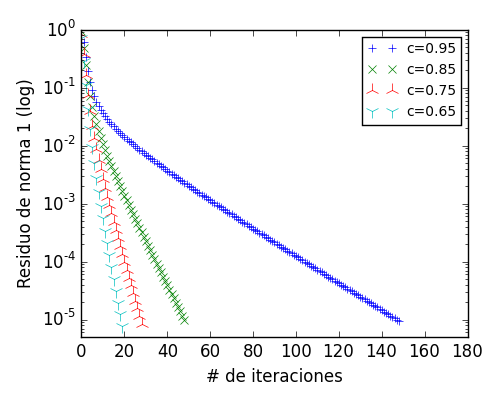
\includegraphics[width=1\textwidth]{imgs/convergencia-stanford.png}
  \caption{\footnotesize{Comparación de la velocidad de convergencia del el método para el dataset web-Stanford.}}
  \label{fig:conv1}
\end{minipage}
\hspace{0.02\textwidth}
\begin{minipage}{0.48\textwidth}
  \centering
    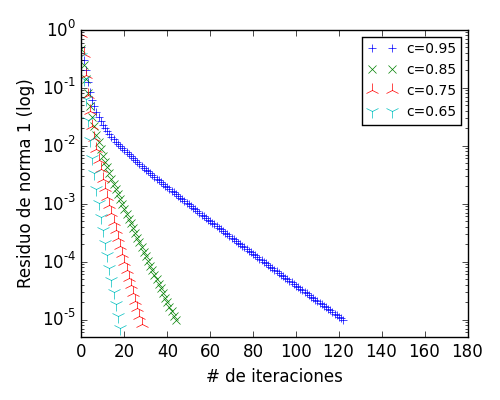
\includegraphics[width=1\textwidth]{imgs/convergencia-notredame.png}
  \caption{\footnotesize{Comparación de la velocidad de convergencia del el método para el dataset web-NotreDame.}}
  \label{fig:conv2}
\end{minipage}
\begin{minipage}{0.5\textwidth}
  \centering
    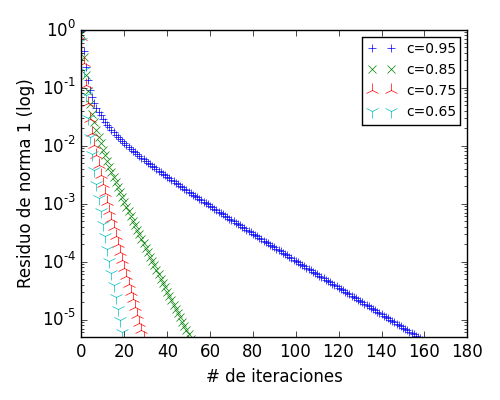
\includegraphics[width=1\textwidth]{imgs/convergencia-google.png}
  \caption{\footnotesize{Comparación de la velocidad de convergencia del el método para el dataset web-Google.}}
  \label{fig:conv3}
\end{minipage}
\end{figure}


Primero notemos algo más o menos sorprendente: la cantidad de iteraciones requeridas por el método no varía demasiado, sobre todo para valores chicos de $c$. Creemos que esto se debe a propiedades generales del método de la potencia, que sin embargo son díficiles de analizar y están fuera del alcance de este trabajo.

Se puede notar además que para los valores más pequeños de $c$ la cantidad de iteraciones correspondientes a cada dataset es prácticamente igual.

Una cosa importante para decir, de la cual vamos a hablar en profundidad más adelante, es que aunque la cantidad de iteraciones sea parecida, el costo de cada iteración es mayor a más grande es la matriz y a más valores no nulos tiene, por lo que las figuras \ref{fig:conv1}, \ref{fig:conv2} y \ref{fig:conv3} no deben intepretarse como el tiempo que requiere el algoritmo para correr.

Sin embargo, una cosa interesante a analizar es qué $c$ usar. Como vimos, usar un $c$ pequeño disminuye el tiempo de cómputo requerido. Sin embargo, disminuir el $c$ también puede impactar en el resultado. Dado que el factor de teletransportación $1-c$ es más alto, de alguna manera el resultado es menos significativo, debido a que se hace más uniforme, como explicamos antes. 
En \cite{Chakrabarti}, por ejemplo, se sugiere que $c$ debería ser elegido basado en la conectividad del grafo.


Otro experimento muy interesante que realizamos es cambiar el criterio de parada del algoritmo iterativo. En particular, lo que hicimos fue cambiar la norma con la que medimos la diferencia entre dos vectores de sucesivas iteraciones. Para ello utilizamos las normas $||-||_1$, $||-||_2$ y $||-||_{\infty}$.

\begin{figure}[H]
\centering

    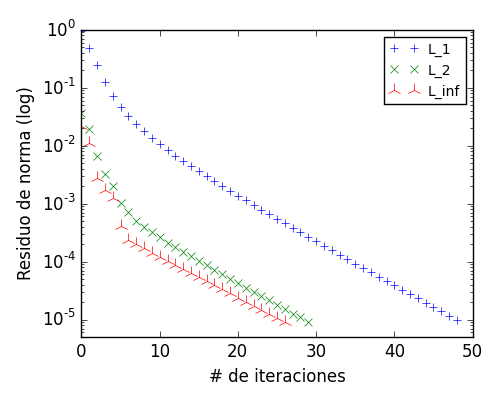
\includegraphics[width=0.6\textwidth]{imgs/convergencia-norma.png}
  \caption{\footnotesize{Comparación de la velocidad de convergencia del el método para el dataset web-Stanford, variando la norma del criterio de parada.}}
  \label{fig:conv-norma}
\end{figure}

Como se observa en la figura \ref{fig:conv-norma}, cuando se utiliza la norma 1 para el criterio de parada, se requieren más iteraciones para terminar. Esto se debe a que la norma 1 es la más \emph{exigente}. 

Se puede probar fácilmente que para todo vector $x$, $||x||_1 \geq ||x||_2 \geq ||x||_{\infty}$ y esto explica claramente los resultados del experimento.



\subsubsection{Rendimiento de PageRank}
A continuación analizaremos el rendimiento del algoritmo de PageRank implementado en este trabajo, es decir, el de \cite{Kamvar2003}. Para ello, utilizaremos los mismos datasets que en la sección anterior.

\begin{figure}[H]
\centering
\begin{tabular}{| c | c | c | c |}
  \hline
  Dataset & Vértices & Aristas & Tiempo (segundos) \\ \hline \hline
  web-Stanford & 281.903 & 2.312.497 & 7.81882 \\ \hline
  web-NotreDame & 325.729 & 1.497.134 & 3.38163 \\ \hline
  web-Google & 916.428 & 5.105.039 & 23.7367 \\ \hline
\end{tabular}

  \caption{\footnotesize{Comparación de los tiempos que requiere el algoritmo para distintos datasets. Fue ejecutado con $c = 0.85$ y $tolerancia = 0.00001$.  Se tomó el promedio de 20 mediciones.}}
  \label{fig:tiempos1}
\end{figure}

Podríamos empezar a sacar conclusiones apresuradas sobre estos datos, pero para que sean más significativos, preferimos realizar otro experimento antes de comenzar el análisis.
Este experimento consiste en dividir el algoritmo en 2: primero el armado de la matriz (recordemos que como representamos la matriz en CRS este no es un paso trivial) y luego el paso de método de la potencia optimizado presentado en \cite{Kamvar2003}.

Esto nos permitirá ver mejor el problema y tener datos más detallados, con el objetivo de poder analizar mejor que es lo que sucede.

\begin{figure}[H]
\centering
\begin{tabular}{| c | c | c | c |}
  \hline
  Dataset & Tiempo total & Armado de matriz & Método de la potencia \\ \hline \hline
  web-Stanford & 7.81882 & 1.8968 & 5.91098 \\ \hline
  web-NotreDame &  3.38163 & 0.978923 & 2.42743 \\ \hline
  web-Google & 23.7367 & 4.30584 & 18.9483 \\ \hline
\end{tabular}

  \caption{\footnotesize{Comparación de los tiempos que requiere el algoritmo para distintos datasets. Fue ejecutado con $c = 0.85$ y $tolerancia = 0.00001$. Se tomó el promedio de 20 mediciones. Todos los tiempos son en segundos. Las sumas probablemente no den bien porque fueron tomadas en diferentes mediciones. }}
  \label{fig:tiempos2}
\end{figure}


Ahora, teniendo toda la información que nos proveen la figura \ref{fig:tiempos1}, \ref{fig:tiempos2} y los experimentos de la sección anterior, podemos hacer un análisis completo y riguroso.

Podemos concluir primero que el paso más costoso del algoritmo es el método de la potencia. Justamente por eso \cite{Kamvar2003} se ocupa de intentar optimizar ese paso, dado que optimizarlo va a impactar fuertemente en el rendimiento general de la aplicación.


Otro aspecto interesante para ver es, como aunque las iteraciones requeridas para cada dataset son bastante similares, el costo de cada operación es muy distinto, pues el tamaño de los vectores varía, y las entradas no nulas de la matriz son distintas. 

De hecho, este experimento nos permite confirmar que el paso más costoso es realizar el producto de la matriz y el vector $P^t x^{(k)}$, ya que se puede ver como el método de la potencia en el caso de web-NotreDame tarda menos que en el caso de web-Stanford, aunque los vectores sean más largos. 

Esto se debe a que la matriz de web-NotreDame es más esparsa, y al multiplicar $Ax$ con $A$ representada en CRS, el costo resulta lineal en la cantidad de elementos no nulos de la matriz. Esta última está intimamente relacionada con la cantidad de aristas del grafo. De esta manera se explica fácilmente el comportamiento a priori extraño de el algoritmo sobre estos datasets.


\subsubsection{Comportamiento de PageRank e In-Deg}

En esta sección estudiaremos como influye la forma de la red de enlaces entre los sitios web en el resultado final de los rankings de PageRank e In-Deg. Veremos las diferencias entre ambos métodos, sus ventajas y desventajas.

Para comenzar nuestra investigación decidimos utilizar un grafo de tan solo 4 nodos, es un ejemplo extraido de \cite{Bryan2006}. Los resultados de pageRank y de In-Deg estan listados mas abajo, pero antes de verlos intentemos analizar que debería suceder. In-Deg decidirá la posición en el ranking de cada sitio web basandose unicamente en la cantidad de links que apunten al mismo por lo que preveer quién quedará primero se reduce a contar los links entrantes, se harán algunas observaciones interesantes de su funcionamiento mas adelante. En el caso de PageRank saber que sitio web tendrá un puesto alto en el ranking no será tan trivial como contar links, para entender mejor los resultados de este método será útil recordar la idea en la que se basa, el modelado de un navegante de la web que recorre cada sitio y donde se cataloga cada página según el tiempo que paso este en cada una.

\begin{figure}[H]
\centering
\begin{tikzpicture}[->,>=stealth',shorten >=1pt,auto,node distance=2.8cm,
                    semithick]
  \tikzstyle{every state}=[fill=red,draw=none,text=white]

	\node[state]			 (A)				 {$A$};
	\node[state]         (B) [below of=A] {$B$};
	\node[state]         (C) [right of=A] {$C$};
	\node[state]         (D) [below of=C] {$D$};
	\path	(A) edge              node {} (B)
            		edge              node {} (C)
            		edge   [bend left]node {} (D)
			(B) edge              node {} (C)        
            		edge              node {} (D)
			(C) edge              node {} (A)
            (D)	edge  [bend left] node {} (A)
            		edge              node {} (C);

\end{tikzpicture}
  \caption{\footnotesize{ Grafo 1: Ejemplo extraido de \cite{Bryan2006} }}
  \label{fig:Rankings}
\end{figure}

Al correr los rankings se nota una gran diferencia de resultados entre cada método.

\begin{figure}[H]
\centering
\begin{tabular}{| c | c | c | c |}
  \hline
  Puestos & PageRank & In-Deg \\ \hline \hline
  1 & A (0.368151) & C \\ \hline
  2 & C (0.287961) & A y D \\ \hline
  3 & D (0.202078) & B\\ \hline
  4 & B (0.14181 ) & None \\ \hline
\end{tabular}

  \caption{\footnotesize{Puestos de cada pagina del Grafo 1 segun PageRank e In-deg}}
  \label{fig:Rankings}
\end{figure}

Para In-Deg como era de esperarse quedó primero el nodo C por tener 3 nodos que lo apuntan, segundos A y D y por último C en tercer lugar. Con pageRank algo que nos llamó la atención al principio fue como terminó quedando en primer lugar el nodo A el cual no parecería, por sus conexiones, ser una página tan relevante, al hacer un análisis de mayor profundidad nos dimos cuenta de una caracteristica importante en la estructura de la red. El nodo C el cual es el que tiene la mayor cantidad de nodos entrantes solo tiene un nodo saliente y este va hacia A, el resultado de esto es que al recorrer la red y llegar a C, a menos que uno se teletransporte, terminará visitando A. Esto provoca que el tiempo que pasa el navegante en C lo pase también en A, agregado a este tiempo el que el navegante pasa de D a A se vuelve entendible que A haya resultado primero.

\paragraph{Generalización del Análisis}

A partir del grafo anterior surgen varias hipótesis sobre las que iremos discutiendo y experimentando en esta sección. Para hacer los experimentos recurriremos a casos simples y claros aunque quizas no lo suficientemente generales como para justificar una demostración totalmente abarcativa de nuestras hipotesis, el objetivo de esta sección será por lo tanto unicamente exponer de forma intuitiva y clara algunas reglas en el funcionamiento de pageRank e In-Deg que hemos observado, las cuales quedarán para demostrarse y generalizarse con mayor profundidad en trabajos futuros. Por ahora nos limitaremos a verificarlas para una cantidad limitada de grafos los cuales se verán mas abajo.

Los grafos que estudiaremos pueden entenderse como un conjunto de nodos con links salientes y entrantes. Dividiremos entonces esta sección en dos para estudiar por separado los efectos de cada uno en los resultados de los rankings.

\paragraph{Links Salientes}
 Lo primero que veremos es como influyen los links salientes de una página $P$ en su posición en el ranking. Creemos que en ambos métodos lo ideal, al menos en teoría, será no tener ningún link saliente ya que en In-Deg al tener enlaces que apunten a otros sitios les estamos dando mayor puntaje lo cual podría ponerlos por encima de nosotros, por otro lado en pageRank si apuntamos a una página (o más) estamos, al igual que pasaba en el Grafo 1, provocando que el navegante cada vez que pase por nuestro espacio pase luego con cierta probabilidad por los otros a los que estamos apuntando, si solo apuntamos a uno o unos pocos nodos entonces le estaremos dando una gran ventaja ya que la probabilidad de que el navegante pase por ellos cada vez que pase por nosotros será alta y en consecuencia la posición en el ranking de estos sitios será favorecida, de aquí deducimos que lo mejor si se quiere apuntar a sitios webs en el caso de PageRank es apuntar a la mayor cantidad posible para no darle mucha ventaja a uno solo sino que esta se disemine, dandole una ventaja minima a cada uno.

La hipotesis sobre In-Deg nos pareció que no requería mayores justificaciones. En el caso de pageRank creamos la siguiente red para verificar lo dicho previamente.

\begin{figure}[H]
\centering
\begin{tikzpicture}[->,>=stealth',shorten >=1pt,auto,node distance=2.8cm,
                    semithick]
  \tikzstyle{every state}=[fill=red,draw=none,text=white]

	\node[state] 		(A)               {$A$};
	\node[state]         (B) [right of=A] {$B$};
	\node[state]         (C) [right of=B] {$C$};
	\node[state]         (D) [above of=B] {$D$};

	\path	(A) edge              node {} (D)
			(B) edge              node {} (D)        
			(C) edge              node {} (D);        


\end{tikzpicture}
  \caption{\footnotesize{ Grafo 2 }}
  \label{fig:Rankings}
\end{figure}

Tenemos, en el Grafo 2, un nodo D el cual está primero tanto para In-Deg como para PageRank.

\begin{figure}[H]
\centering
\begin{tabular}{| c | c | c | c |}
  \hline
  Puestos & PageRank\\ \hline \hline
  1 & D (0.541986)\\ \hline
  2 & A, B y C(0.152671)\\ \hline
\end{tabular}
  \caption{\footnotesize{Puestos de cada pagina del grafo1 segun PageRank e In-deg}}
  \label{fig:Rankings}
\end{figure}

Veamos que pasa cuando agregamos un nodo más de la siguiente manera.

\begin{figure}[H]
\centering
\begin{tikzpicture}[->,>=stealth',shorten >=1pt,auto,node distance=2.8cm,
                    semithick]
  \tikzstyle{every state}=[fill=red,draw=none,text=white]

	\node[state] 		(A)               {$A$};
	\node[state]         (B) [right of=A] {$B$};
	\node[state]         (C) [right of=B] {$C$};
	\node[state]         (D) [above of=B] {$D$};
	\node[state]         (E) [above of=D] {$E$};
%	\node[state]         (F) [above of=E]       {$D_n$};

	\path	(A) edge              node {} (D)
			(B) edge              node {} (D)        
			(C) edge              node {} (D)        
			(D) edge              node {} (E);
%	\path[->, dotted] (E) edge	node {} (F);
%	\path[->, dotted] (I) edge	node {} (D);        
\end{tikzpicture}
  \caption{\footnotesize{ Grafo 3 }}
  \label{fig:Rankings}
\end{figure}

\begin{figure}[H]
\centering
\begin{tabular}{| c | c | c | c |}
  \hline
  Puestos & PageRank\\ \hline \hline
  1 & E (0.380177)\\ \hline
  2 & D (0.335934)\\ \hline
  3 & A, B y C(0.0946297)\\ \hline
\end{tabular}
  \caption{\footnotesize{Puesto de cada nodo del grafo 3}}
  \label{fig:Rankings}
\end{figure}

Al hacer esto ocurre lo predicho, el navegante, a menos que se teletransporte, pasara por E siempre, sumando a esto las veces que visita directamente a E debido a una teletransportación se vuelve entendible por que D esta ahora en segundo lugar. Veamos como podemos mejorar esta situación, claramente si cortamos el enlace a E volveremos a la situación previa donde estaba primero pero de ser esto imposible creemos que lo mejor que puede hacer el nodo D es conectarse a la mayor cantidad de páginas posibles, ya que asi podría lograr difuminar la ventaja que le da a cada sitio web. Para comprobar esto armamos los grafos 4 y 5.

\begin{figure}[H]
\centering
\begin{tabular}{| c | c | c | c |}
  \hline
  Puestos & In-Deg\\ \hline \hline
  1 & D\\ \hline
  2 & E\\ \hline
  3 & A, B y C\\ \hline
\end{tabular}
  \caption{\footnotesize{Ranking del grafo 3 con In-Deg}}
  \label{fig:Rankings}
\end{figure}


Es interesante contrastar este resultado con el que tendría In-Deg, para el grafo 3 obtenemos en primer lugar a D, esto sucede debido a que este método supone que tener una gran cantidad de sitios apuntandote es lo mas importante sin preocuparse por quienes sean los sitios en sí. Esta caracteristica es la que vuelve a In-Deg irrealista ya que no modela la diferencia entre un sitio apuntado por 3 nodos aislados y uno apuntado por 3 sitios de gran trayectoria.

\begin{figure}[H]
\centering
\begin{minipage}{0.48\textwidth}
  \centering
\begin{tikzpicture}[->,>=stealth',shorten >=1pt,auto,node distance=2.8cm,
                    semithick]
  \tikzstyle{every state}=[fill=red,draw=none,text=white]

	\node[state] 		(A)               {$A$};
	\node[state]         (B) [right of=A] {$B$};
	\node[state]         (C) [right of=B] {$C$};
	\node[state]         (D) [above of=B] {$D$};
	\node[state]         (E) [above left of=D] {$E$};
	\node[state]         (F) [above right of=D] {$F$};

	\path	(A) edge              node {} (D)
			(B) edge              node {} (D)        
			(C) edge              node {} (D)        
			(D) edge              node {} (E)
			(D) edge              node {} (F);
\end{tikzpicture}
  \caption{\footnotesize{ Grafo 4 }}
  \label{fig:Rankings}

\end{minipage}
\hspace{0.02\textwidth}
\begin{minipage}{0.48\textwidth}
  \centering

\begin{tikzpicture}[->,>=stealth',shorten >=1pt,auto,node distance=2.8cm,
                    semithick]
  \tikzstyle{every state}=[fill=red,draw=none,text=white]

	\node[state] 		(A)               {$A$};
	\node[state]         (B) [right of=A] {$B$};
	\node[state]         (C) [right of=B] {$C$};
	\node[state]         (D) [above of=B] {$D$};
	\node[state]         (E) [above left of=D] {$E$};
	\node[state]         (F) [above of=D] {$F$};
	\node[state]         (G) [above right of=D] {$G$};

	\path	(A) edge              node {} (D)
			(B) edge              node {} (D)        
			(C) edge              node {} (D)        
			(D) edge              node {} (E)
			(D) edge              node {} (F)
			(D) edge              node {} (G);
		
\end{tikzpicture}
  \caption{\footnotesize{ Grafo 5 }}
  \label{fig:Rankings}

\end{minipage}
\end{figure}

Se puede ver como al apuntar D a mas sitios su supremacia se vuelve a reestablecer cada vez mas mientras mayor es la cantidad de nodos a los que apunta, corroborando lo dicho previamente.

\begin{figure}[H]
\centering
\begin{minipage}{0.48\textwidth}
\centering

\begin{tabular}{| c | c | c | c |}
  \hline
  Puestos & PageRank\\ \hline \hline
  1 & D (0.306893)\\ \hline
  2 & E y F (0.21688)\\ \hline
  3 & A, B y C(0.0864493)\\ \hline
\end{tabular}
  \caption{\footnotesize{Puesto de cada nodo del grafo 4}}
  \label{fig:Rankings}

\end{minipage}
\hspace{0.02\textwidth}
\begin{minipage}{0.48\textwidth}
  \centering

\begin{tabular}{| c | c | c | c |}
  \hline
  Puestos & PageRank\\ \hline \hline
  1 & D (0.282476)\\ \hline
  2 & E, F y G (0.159605)\\ \hline
  3 & A, B y C(0.0795699)\\ \hline
\end{tabular}
  \caption{\footnotesize{Puesto de cada nodo del grafo 5}}
  \label{fig:Rankings}

\end{minipage}
\end{figure}


\paragraph{Links Entrantes}

En el caso de In-Deg sale directamente de su definición como la cantidad de links entrantes decide la posición en el ranking de cada nodo. En el caso de PageRank la cantidad de páginas entrantes a un nodo creemos que tambien ayudara a este a ponerlo en una mejor posición aunque el nivel de ayuda que estos enlaces brinden dependerá de la importancia de las páginas de las cuales provengan y si estan apuntando a otros nodos o no. Analizar esto es como analizar lo discutido en la sección anterior desde el punto de vista inverso. Es decir, en el experimento anterior vimos que cada vez que D apuntaba a mas sitios la posición en el ranking de las páginas a las que apuntaba bajaba mas, a partir de eso, se deduce de forma inmediata que si queremos tener un ranking alto será importante no solo que nos apunten sino también que lo hagan con un grado de exclusividad lo mas alto posible.

En este grafo intentamos verificar lo dicho, conjeturando que, a diferencia de lo que pasaría con In-Deg, con PageRank el nodo G saldrá mejor que el H y F a pesar de tener la misma cantidad de enlaces apuntandolos, debido a que H y F comparten los nodos entrantes a diferencia de G que los tiene exclusivamente para el.
\begin{figure}[H]
\centering
\begin{tikzpicture}[->,>=stealth',shorten >=1pt,auto,node distance=2.8cm,
                    semithick]
  \tikzstyle{every state}=[fill=red,draw=none,text=white]

	\node[state] 		(A)               {$A$};
	\node[state]         (B) [right of=A] {$B$};
	\node[state]         (C) [right of=B] {$C$};
	\node[state]         (D) [right of=C] {$D$};
	\node[state]         (E) [right of=D] {$E$};
	\node[state]         (F) [right of=E] {$F$};
	\node[state]         (G) [above of=B] {$G$};
	\node[state]         (H) [above right of=D] {$H$};
	\node[state]         (I) [above left of=F] {$I$};


	\path	(A) edge              node {} (G)
			(B) edge              node {} (G)        
			(C) edge              node {} (G)        
			(D) edge              node {} (I)        
			(E) edge              node {} (I)        
			(F) edge              node {} (I)        
			(D) edge              node {} (H)        
			(E) edge              node {} (H)        
			(F) edge              node {} (H);        


\end{tikzpicture}
  \caption{\footnotesize{ Grafo 6 }}
  \label{fig:Rankings}
\end{figure}

\begin{figure}[H]
\centering
\begin{tabular}{| c | c | c | c |}
  \hline
  Puestos & PageRank\\ \hline \hline
  1 & G (0.251774)\\ \hline
  2 & H e I (0.161348)\\ \hline
  3 & A, B, C, D, E y F (0.0709217)\\ \hline
\end{tabular}
  \caption{\footnotesize{Ranking del grafo 7}}
  \label{fig:Rankings}
\end{figure}

